% !TEX root = mth727_lecture_notes.tex


\chapter[Higher Homotopy Groups]{Higher Homotopy \\ Groups}
\chaptermark{Higher Homotopy Groups}
\label{HIGHER HOMOTOPY GROUPS CHAPTER}
\thispagestyle{firststyle}


\begin{notation}\ 
\benu
\item[] $I^{n} = \{(s_{1}, \dots, s_{n}) \ |\  s_{i}\in [0, 1], i=1, \dots, n \}$
\item[] $\partial I^{n} = \{(s_{1}, \dots, s_{n}) \in I^{n} \ |\  
s_{i}\in \{0, 1\} \text{ for some } i \}$
\item[] $D^{n} = \{(x_{1}, \dots x_{n})\in \R^{n} \ | \  \sum_{i}x^{2}_{i} \leq 1 \}$
\item[] $S^{n-1} = \{(x_{1}, \dots x_{n})\in \R^{n} \ | \  \sum_{i}x^{2}_{i} = 1 \}$
\eenu
\end{notation}


\vskip -3mm
Recall that the fundamental group $\pi_{1}(X, x_{0})$ of a pointed space $(X, x_{0})$
is the group whose elements are homotopy classes of maps $\omega: (I, \pint) \to (X, x_{0})$. 
Multiplication is given by concatenation of such maps.

\vskip -2mm
\begin{equation*}
\begin{tikzpicture}[
    scale = 1,
    d0/.style = {line width = 1.6pt},
    d1/.style= {postaction={decorate}, line width = 1.6pt, decoration={markings, mark=at position 0.55 with {\arrow[rotate=-2]{stealth}}}},
    d2/.style = {postaction={decorate}, line width = 1.6pt, decoration={markings, mark=at position 0.54 with {\arrow[rotate=4]{stealth}}}}
]

\draw[d0, red] (0,0) -- node[anchor=south, yshift = 2pt] {\small $\omega$} (1.5, 0); 
\draw[d0, myblue] (1.5,0) --  node[anchor=south, yshift = 2pt] {\small $\tau$} (3, 0); 
\filldraw (0,0) circle (0.08) node[anchor = north, yshift = -2pt] {\small $0$};
\filldraw (1.5,0) circle (0.08) node[anchor = north, yshift = -2pt] {\small $\frac{1}{2}$};
\filldraw (3,0) circle (0.08) node[anchor = north, yshift = -2pt] {\small $1$};

\draw[thick, ->, >=latex] (3.7, 0) -- node[anchor= south] {\small $\omega\ast \tau$}(4.9, 0);


\begin{scope}[scale=0.6, xshift = 320pt]
\draw[fill = mygray1] (-2.2, -2.2) rectangle (3.5, 2.2);
\draw[d0, red, rotate=25, , yscale = 0.9]  
(0,0) .. controls (0,0) and (1,1) .. 
(2, 1) .. controls (2.5,1) and (3, 0.5).. 
(3,0)  ..controls (3, -0.5) and (2.5, -1)..  
(2,-1) ..controls (1, -1) and (0,0).. 
cycle;
\node[red] at (2.5, -0.2)  {\small $\omega$} ;

\draw[d0, myblue, rotate = -135, scale = 0.7]
(0,0) .. controls (0,0) and (1,1) .. 
(2, 1) .. controls (2.5,1) and (3, 0.5).. 
(3,0)  ..controls (3, -0.5) and (2.5, -1)..  
(2,-1) ..controls (1, -1) and (0,0).. 
cycle; 
\node[myblue] at (0.05, -1.3)  {\small $\tau$} ;

\draw[fill = black] (0,0) circle (0.12) node[anchor=south east] {\small $x_{0}$};
\node[anchor = north west] at (-2.2, 2.2) {\small $X$};

\end{scope}
\end{tikzpicture}
\end{equation*}

Alternatively, $\pi_{1}(X, x_{0})$ can be described as a group whose elements are homotopy 
classes of maps $\omega \colon (S^{1}, s_{0}) \to (X, x_{0})$. In this setting, 
the multiplication in $\pi_{1}(X, x_{0})$ is defined using the pinch map 
$p\colon S^{1} \to S^{1}\vee S^{1}$:

\vskip -2mm
\begin{equation*}
\begin{tikzpicture}[
    scale = 0.6,
    d0/.style = {line width = 1.6pt},
    d1/.style= {postaction={decorate}, line width = 1.6pt, decoration={markings, mark=at position 0.55 with {\arrow{stealth}}}},
    d2/.style = {postaction={decorate}, line width = 1.6pt, decoration={markings, mark=at position 0.54 with {\arrow[rotate=-9]{stealth}}}},
]

\begin{scope}
\draw[d2, red] (1,0) arc (0:180:1);
\draw[d2, myblue] (-1,0) arc (180:360:1);
\draw[fill = black] (-1,0) circle (0.12);
\draw[fill = black] (1,0) circle (0.12);
\end{scope}

\begin{scope}[xshift = 21mm]
\draw[thick, ->, >=latex] (0,0) -- node[anchor=south] {\small $p$} (1.5,0);
\end{scope}


\begin{scope}[xshift = 55 mm]
\draw[opacity = 0] (0 , -2.2) -- (0, 2.2); % dummy so that arrow on circle show
\draw[d2, red] (0,0) arc (-90:270:1);
\draw[d2, myblue] (0,0) arc (90:450:1);
\draw[fill = black] (0,0) circle (0.12);
\end{scope}

\begin{scope}[xshift = 75mm]
\draw[thick, ->, >=latex] (0,0) -- node[anchor=south] {\small $\omega\vee \tau$} (2,0);
\end{scope}


\begin{scope}[xshift = 130 mm]
\draw[fill = mygray1] (-2.2, -2.2) rectangle (3.5, 2.2);
\draw[d0, red, rotate=25, , yscale = 0.9]  
(0,0) .. controls (0,0) and (1,1) .. 
(2, 1) .. controls (2.5,1) and (3, 0.5).. 
(3,0)  ..controls (3, -0.5) and (2.5, -1)..  
(2,-1) ..controls (1, -1) and (0,0).. 
cycle;
\node[red] at (2.5, -0.2)  {\small $\omega$} ;

\draw[d0, myblue, rotate = -135, scale = 0.7]
(0,0) .. controls (0,0) and (1,1) .. 
(2, 1) .. controls (2.5,1) and (3, 0.5).. 
(3,0)  ..controls (3, -0.5) and (2.5, -1)..  
(2,-1) ..controls (1, -1) and (0,0).. 
cycle; 
\node[myblue] at (0.05, -1.3)  {\small $\tau$} ;

\draw[fill = black] (0,0) circle (0.12) node[anchor=south east] {\small $x_{0}$};
\node[anchor = north west] at (-2.2, 2.2) {\small $X$};

\end{scope}
\end{tikzpicture}
\end{equation*}


This construction can be generalized to define higher homotopy groups. 


\begin{definition/proposition}
\label{HIGHER HOMOT GPS DEF}
Let $(X, x_{0})$ be a pointed space. For $n\geq 1$ the \emph{$n$-th homotopy group} of 
$(X, x_{0})$ is the group $\pi_{n}(X, x_{0})$ whose elements are homotopy classes 
of maps $\omega\colon (I^{n}, \pint^{n}) \to (X, x_{0})$. Multiplication in 
$\pi_{n}(X, x_{0})$ is defined as follows. 
If $\omega, \tau\colon (I^{n}, \pint^{n}) \to (X, x_{0})$ then 
\[[\omega]\cdot [\tau] = [\omega\ast\tau]\]
where $\omega\ast\tau\colon (I^{n}, \pint^{n}) \to (X, x_{0})$ is given by 
\[
(\omega\ast \tau)(s_{1}, s_{2}, \dots, s_{n}) = 
\begin{cases}
\omega(2s_{1}, s_{2}, \dots, s_{n}) & \text{ for } s_{1}\in [0, \frac{1}{2}] \\
\tau(2s_{1} -1, s_{2}, \dots, s_{n}) & \text{ for } s_{1}\in [\frac{1}{2}, 1] \\
\end{cases}
\]

\begin{equation*}
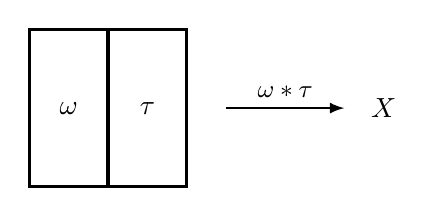
\begin{tikzpicture}
\draw[very thick] (0,0) rectangle  node[anchor=center] {$\omega$} (1,2);
\draw[very thick] (1,0) rectangle node[anchor=center] {$\tau$}(2,2);

\draw[thick, ->, >=latex] (2.5, 1) -- node[anchor=south] {\small $\omega\ast\tau$} (4.0,1);
\node at (4.5, 1) {$X$};
\end{tikzpicture}
\end{equation*}
The trivial element 
of $\pi_{n}(X, x_{0})$ is the homotopy class of the constant map $c_{x_{0}}\colon I^{n} \to X$. Also, for 
$[\omega]\in \pi_{1}(X, x_{0})$ we have $[\omega]^{-1} = [\xov{\omega}]$ where 
$\xov{\omega}\colon  (I^{n}, \partial I^{n}) \to (X, x_{0})$ is given by 
\[
\xov{\omega}(s_{1}, s_{2}, \dots, s_{n}) = \omega(1-s_{1}, s_{2}, \dots, s_{n})\
\]
\end{definition/proposition}

\begin{note}
A part of Definition \ref{HIGHER HOMOT GPS DEF} makes sense also for $n=0$. 
In this case we have $I^{0} = \{\ast\}$ and $\partial I^{0} = \varnothing$. 
We define $\pi_{0}(X, x_{0})$ as the set of homotopy classes of maps 
$\omega \colon (I^{0}, \partial I^{0}) \to (X, x_{0})$.  
Giving such a map is the same as selecting a point
$\omega(\ast) = x_{\omega} \in X$. Giving a homotopy of such maps is equivalent to giving
a path between the corresponding points. Thus two points $x_{\omega}$ and 
$x_{\tau}$ represent the same element of $\pi_{0}(X, x_{0})$ if they belong to
the same path connected component. In other words, we get 
\[
\pi_{0}(X, x_{0}) \ \cong \  
\begin{pmatrix}
\text{path connected} \\[1mm]
\text{components of $X$} \\
\end{pmatrix} 
\]
The trivial element of $\pi_{0}(X, x_{0})$ is given by the map $c_{x_{0}}\colon I^{0} \to X$
such that $c_{x_{0}}(\ast) = x_{0}$. This corresponds to the path connected component 
of $x_{0}$ in $X$. In this way  $\pi_{0}(X, x_{0})$ becomes a pointed set. There is no 
multiplication defined in $\pi_{0}(X, x_{0})$.
\end{note}


\begin{theorem}
\label{HIGHER HOMOT GPS ABELIAN THM}
For $n\geq 2$ then the group $\pi_{n}(X, x_{0})$ is abelian for any  pointed space 
$(X, x_{0})$.   
\end{theorem}

\begin{proof}[Pictorial proof]
A homotopy $\omega\ast\tau \simeq \tau\ast\omega$ can be depicted as follows:

\begin{equation*}
\begin{tikzpicture}
\draw[very thick] (0,0) rectangle  node[anchor=center] {$\omega$} (1,2);
\draw[very thick] (1,0) rectangle node[anchor=center] {$\tau$}(2,2);
\node at (2.5,1) {$\simeq$};
\draw[very thick] (3,0) rectangle  node[anchor=center] {$\omega$} (4,1);
\draw[very thick] (4,1) rectangle node[anchor=center] {$\tau$}(5,2);
\draw[very thick, fill=mygray2] (3,1) rectangle node[anchor=center] {$x_{0}$}(4,2);
\draw[very thick,  fill=mygray2] (4,0) rectangle node[anchor=center] {$x_{0}$}(5,1);
\node at (5.5,1) {$\simeq$};
\draw[very thick] (6,0) rectangle  node[anchor=center] {$\omega$} (8,1);
\draw[very thick] (6,1) rectangle node[anchor=center] {$\tau$}(8,2);
\node at (8.5,1) {$\simeq$};
\draw[very thick,  fill=mygray2] (9,0) rectangle  node[anchor=center] {$x_{0}$} (10,1);
\draw[very thick,  fill=mygray2] (10,1) rectangle node[anchor=center] {$x_{0}$}(11,2);
\draw[very thick] (9,1) rectangle node[anchor=center] {$\tau$}(10,2);
\draw[very thick] (10,0) rectangle node[anchor=center] {$\omega$}(11,1);
\node at (11.5,1) {$\simeq$};
\draw[very thick] (12,0) rectangle  node[anchor=center] {$\tau$} (13,2);
\draw[very thick] (13,0) rectangle node[anchor=center] {$\omega$}(14,2);
\end{tikzpicture}
\end{equation*}
The shaded squares in the pictures are mapped to the basepoint $x_{0}\in X$.
\end{proof}

A more rigorous proof can be obtained using the following fact.

\begin{ECKMAN-HILTON THM}
\label{ECKMANHILTON THM}
Let $M$ be a set equipped with two binary operations
\[\circ \colon M \times M \to M, \ \ \ \bullet \colon M \times M \to M\]
Assume that there  exist elements $1_{\circ}, 1_{\bullet} \in M$ such that 
$m \circ 1_{\circ} =  1_{\circ}\circ m = m$ and 
$m \bullet 1_{\bullet} =  1_{\bullet}\bullet m = m$
for all $m\in M$. Assume also, that for any $m_{1}, m_{2}, n_{1}, n_{2}\in M$ we have
\[
(m_{1}\circ m_{2}) \bullet (n_{1}\circ n_{2}) = 
(m_{1}\bullet n_{1})\circ (m_{2}\bullet n_{2})
\]
Then for any $m, n\in M$ we have $m\circ n = m\bullet n$, and $m\circ n = n \circ m$.
\end{ECKMAN-HILTON THM}

\begin{proof}
Exercise.
\end{proof}


\begin{proof}[Proof of Theorem \ref{HIGHER HOMOT GPS ABELIAN THM}]
Recall that  multiplication in $\pi_{n}(X, x_{0})$ is defined by 
If $\omega, \tau\colon (I^{n}, \pint^{n}) \to (X, x_{0})$ then 
\[[\omega]\cdot [\tau] = [\omega\ast\tau]\]
where $\omega\ast\tau\colon (I^{n}, \pint^{n}) \to (X, x_{0})$ is given by 
\[
(\omega\ast \tau)(s_{1}, s_{2}, \dots, s_{n}) = 
\begin{cases}
\omega(2s_{1}, s_{2}, \dots, s_{n}) & \text{ for } s_{1}\in [0, \frac{1}{2}] \\
\tau(2s_{1} -1, s_{2}, \dots, s_{n}) & \text{ for } s_{1}\in [\frac{1}{2}, 1] \\
\end{cases}
\] 
\begin{equation*}
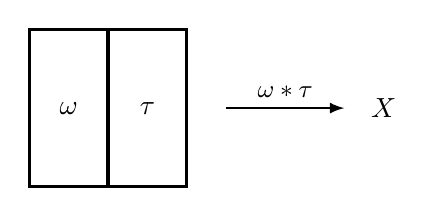
\begin{tikzpicture}
\draw[very thick] (0,0) rectangle  node[anchor=center] {$\omega$} (1,2);
\draw[very thick] (1,0) rectangle node[anchor=center] {$\tau$}(2,2);

\draw[thick, ->, >=latex] (2.5, 1) -- node[anchor=south] 
{\small $\omega\ast\tau$} (4.0,1);
\node at (4.5, 1) {$X$};
\end{tikzpicture}
\end{equation*}

Since $n\geq 2$, we can also define a multiplication in $\pi_{n}(X, x_{0})$
by 
\[
[\omega]\odot [\tau] = [\omega\circledast\tau]
\]
where
\[
(\omega\circledast \tau)(s_{1}, s_{2}, \dots, s_{n}) = 
\begin{cases}
\omega(s_{1}, 2s_{2}, \dots, s_{n}) & \text{ for } s_{2}\in [0, \frac{1}{2}] \\
\tau(s_{1}, 2s_{2} - 1, \dots, s_{n}) & \text{ for } s_{2}\in [\frac{1}{2}, 1] \\
\end{cases}
\]
\begin{equation*}
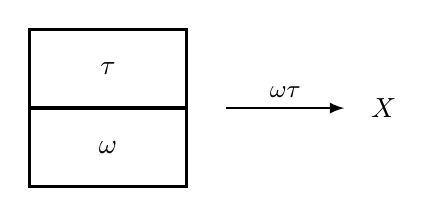
\begin{tikzpicture}
\draw[very thick] (0,0) rectangle  node[anchor=center] {$\omega$} (2,1);
\draw[very thick] (0,1) rectangle node[anchor=center] {$\tau$}(2,2);

\draw[thick, ->, >=latex] (2.5, 1) -- node[anchor=south] {\small $\omega\circledast\tau$} (4.0,1);
\node at (4.5, 1) {$X$};
\end{tikzpicture}
\end{equation*}
Notice that for any 
$\omega_{1}, \omega_{2}, \tau_{1}, \tau_{2}\colon (I^{n}, \pint^{n})\to (X, x_{0})$
we have 
\[(\omega_{1}\ast \omega_{2}) \circledast (\tau_{1}\ast \tau_{2})
= (\omega_{1}\circledast \tau_{1}) \ast (\omega_{2}\circledast \tau_{2})
\]
\begin{equation*}
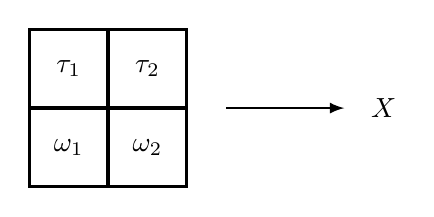
\begin{tikzpicture}
\draw[very thick] (0,0) rectangle  node[anchor=center] {$\omega_{1}$} (1,1);
\draw[very thick] (1,0) rectangle node[anchor=center] {$\omega_{2}$}(2,1);
\draw[very thick] (0,1) rectangle node[anchor=center] {$\tau_{1}$}(1,2);
\draw[very thick] (1,1) rectangle node[anchor=center] {$\tau_{2}$}(2,2);
\draw[thick, ->, >=latex] (2.5, 1) -- (4.0,1);
\node at (4.5, 1) {$X$};
\end{tikzpicture}
\end{equation*}
The result follows from Theorem \ref{ECKMANHILTON THM}.
\end{proof}


\begin{nn} {\bf Alternative construction.}
Just as for the fundamental group, higher homotopy groups can be also 
described using maps from spheres. Since $I^{n}/\pint^{n} \cong S^{n}$, giving 
a map $(I^{n}, \pint^{n}) \to (X, {x_{0}})$ is equivalent to giving a map 
$(S^{n}, s_{0}) \to (X, x_{0})$ for some basepoint $s_{0}\in S^{n}$. Thus 
elements of $\pi_{n}(X, x_{0})$ can be described as homotopy classes of such maps.

To describe multiplication in $\pi_{n}(X, x_{0})$ in this setting,  
consider the pinch map $p\colon S^{n}\to S^{n}\vee S^{n}$ that maps the upper 
hemisphere of $S^{n}$ onto one copy of $S^{n} \subseteq S^{n}\vee S^{n}$, the lower 
hemisphere onto the second copy, and the equator of $S^{n}$ to the basepoint of 
$S^{n}\vee S^{n}$:


\begin{tikzpicture}
\node[anchor=south west,inner sep=0] at (0,0) 
{{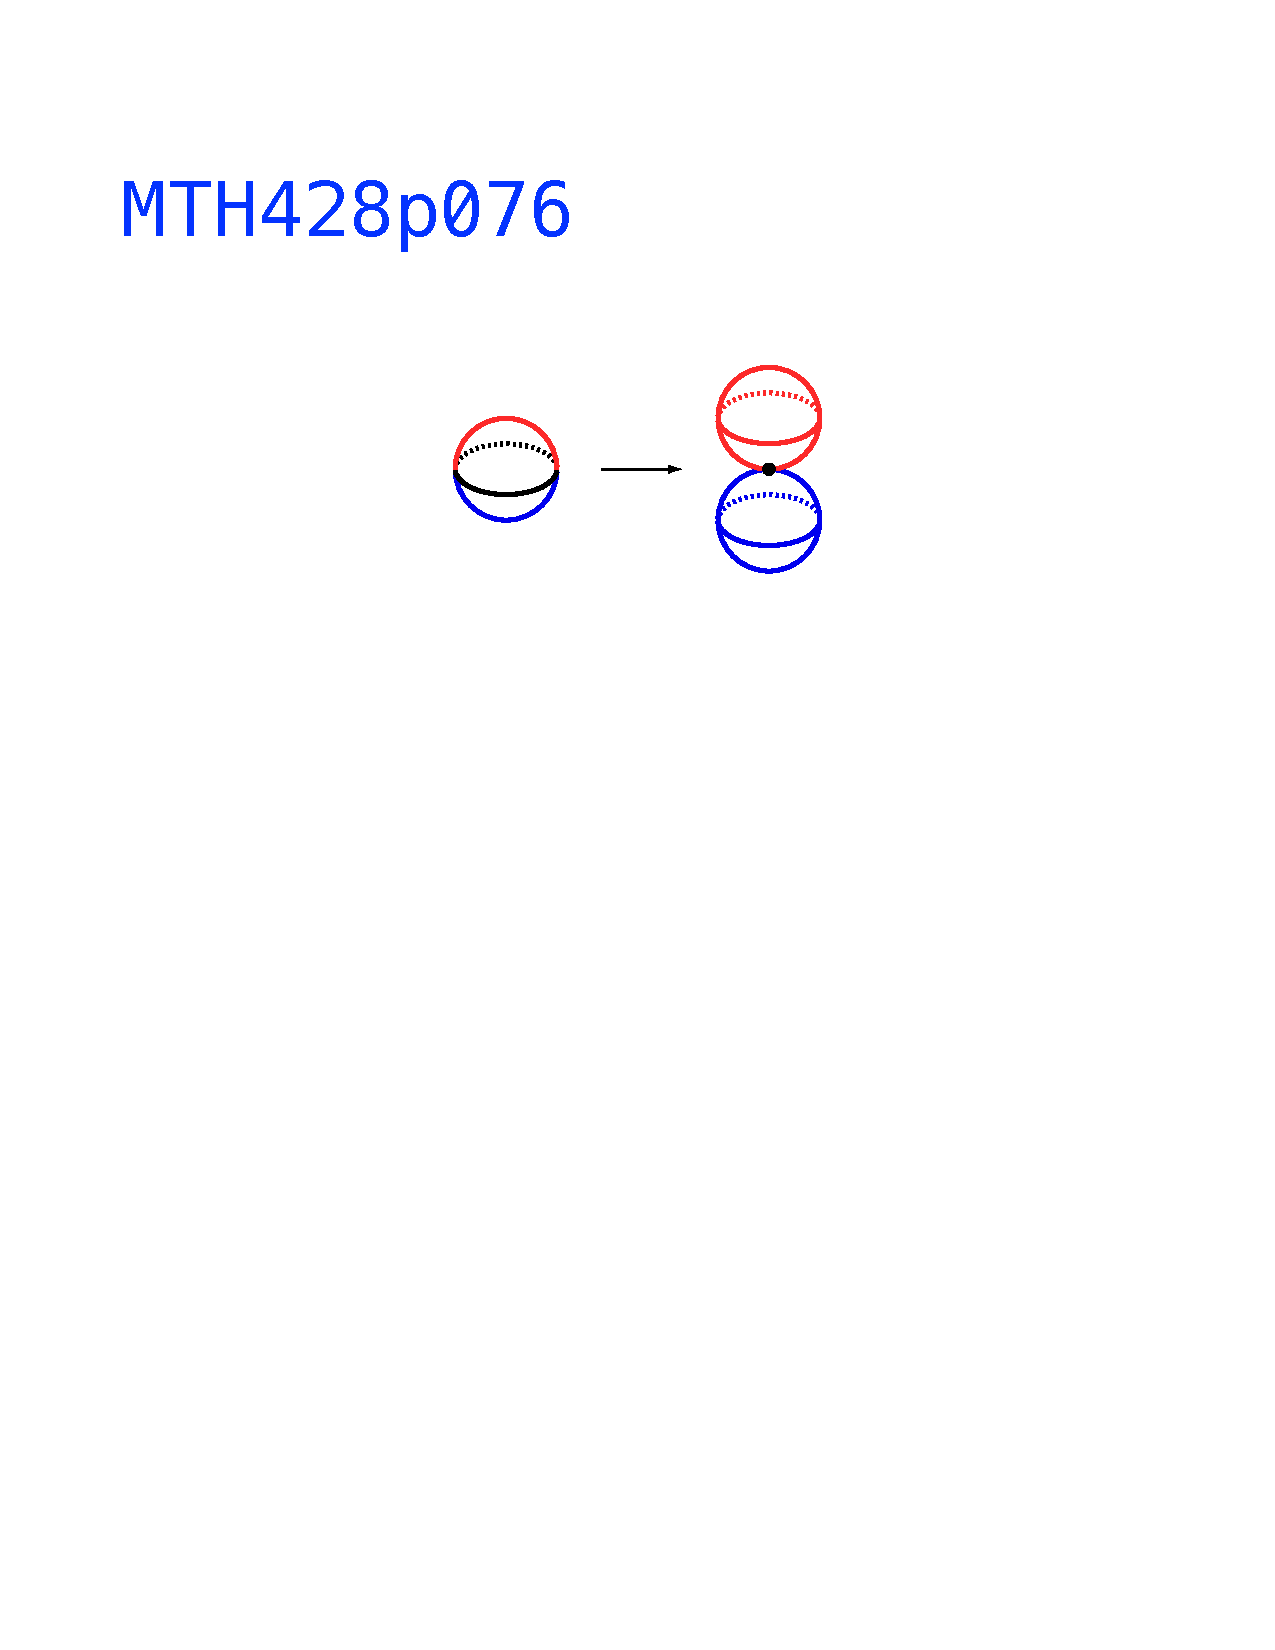
\includegraphics[width=\textwidth, trim=0mm 182mm 0mm 61mm, clip]{pictures/MTH428p076.pdf}}};

%%% COORDINATE GRID
%\draw[step=0.5, help lines] (0,0) to[grid with coordinates] (15,9);
%%% 
\node[anchor= base]  at (8.4 , 1.8){\small  $p$};

\end{tikzpicture}

Given two basepoint preserving maps $\omega, \tau\colon (S^{n}, s_{0}) \to (X, x_{0})$,  
let $\omega\vee \tau \colon S^{n}\vee S^{n} \to X$ be the function that maps the first 
copy of $S^{n}$ using $\omega$ and the second copy using $\tau$. Then we have
\[
[\omega]\cdot [\tau] = [(\omega\vee \tau) \circ p]
\]
\end{nn}


The following fact is often useful:

\begin{proposition}
\label{PIN TRIVAL ELT}
A map $\omega \colon (S^{n}, s_{0}) \to (X, x_{0})$ represents the trivial 
element of $\pi_{n}(X, x_{0})$ if and only if there exists a map 
$\omega’\colon D^{n+1} \to X$ such that $\omega’|_{S^{n}} = \omega$.
\end{proposition}

\begin{proof}
Exercise.
\end{proof}


\begin{nn} {\bf Functoriality.}
Let $f\colon (X, x_{0}) \to (Y, y_{0})$ be a map of pointed spaces. 
For any $\omega\colon (I^{n}, \pint^{n})\to (X, x_{0})$, composition with 
$f$ gives a map $f\circ \omega \colon (I^{n}, \pint^{n}) \to (Y, y_{0})$. 
If $\omega,  \tau \colon (I^{n}, \pint^{n})\to (X, x_{0})$ and $\omega \simeq \tau$, 
then $f\circ \omega\simeq f\circ \tau$. Therefore we get a well defined function
\[
f_{\ast}\colon \pi_{n}(X, x_{0}) \to \pi_{n}(Y, y_{0})
\]
given by $f_{\ast}([\omega]) = [f\circ \omega ]$. If $n\geq 0$ then  $f_{\ast}$
is a homomorphism of groups. For maps $f\colon (X, x_{0}) \to (Y, y_{0})$
and $g\colon (Y, y_{0}) \to (Z, z_{0})$ we have $(gf)_{\ast} = g_{\ast}f_{\ast}$. 
Also, if $\id_{X}\colon (X, x_{0}) \to (X, x_{0})$ is the identity map, then
$\id_{X\ast}\colon \pi_{n}(X, x_{0}) \to \pi_{n}(X, x_{0})$ is the identity homomorphism. 
This shows that the assignments $(X, x_{0})\to \pi_{n}(X, x_{0})$ define functors:
\begin{align*}
\pi_{0}\colon \Top_{\ast} \to &\ \  \Set_{\ast} \\
\pi_{1}\colon \Top_{\ast} \to &\ \  \Gr  \\
\pi_{n}\colon \Top_{\ast} \to &\ \  \Ab  \\
\end{align*}
\vskip -8mm
for $n\geq 2$, where $\Top_{\ast}$ is the category of pointed topological spaces, 
and $\Set_{\ast}$, $\Gr$, $\Ab$ are the categories of pointed sets, groups, and 
abelian groups, respectively.

As a consequence, if $f\colon (X, x_{0}) \to (Y, y_{0})$ is a homeomorphism, 
then $f_{\ast}\colon \pi_{n}(X, x_{0}) \to \pi_{n}(Y, y_{0})$ is an isomorphism 
for $n\geq 0$. 
\end{nn}




